\pagestyle{empty} % Limpa o cabeçalho e o rodapé
\onehalfspacing % Espaçamento entre-linhas de 1,5
% \hyphenpenalty=10000 % To prevent hyphenation
\pretolerance=10000 % To avoid overfull lines
%\selectlanguage{english}
\selectlanguage{brazilian}
%\pagenumbering{arabic} % Uncomment this line if you want renumber pages for each chapter
\setcounter{ex}{0} % counter for exercises
\renewcommand{\chaptername}{Tutorial}
\chapter{Espaço de topologias}\label{tut3}
\rhead{\tiny Instituto de Biociências --USP: BIZ0433 - Inferência Filogenética: Filosofia, Método e Aplicações}
\cfoot{\tiny \cc \ccby \ccsa \href{http://creativecommons.org/licenses/by-sa/4.0/}{Creative Commons Attribution-ShareAlike 4.0 International License}}
%\vspace{5pt}
{\large \sc BIZ0433 - Inferência Filogenética: Filosofia, Método e Aplicações.}\par
%\vspace{10pt}
\par
\minitoc % for table of contents within the chapter
\newpage
\section*{}\addcontentsline{toc}{section}{Objetivo}
\onehalfspacing
\vspace*{5pt}
\begin{center}
\emph{\begin{large}Objetivo\end{large}}\label{tut3:Objetivo}
\vspace{2pt}
\end{center}
%% TEXTO DO RESUMO
Este tutorial apresenta os conceitos de grafos, enumeração e espaço de topologias. O objetivo do tutorial é apresentar os requisitos necessários para a compreensão da complexidade computacional associada às buscas de topologias de acordo com critérios de otimalidade. Durante o tutorial, você terá a oportunidade de executar uma série de exercícios cujos resultados gráficos lhe permitirão adquirir uma melhor compreensão dos conceitos em discussão. Os arquivos associados a este tutorial estão disponíveis no \href{https://github.com/fplmarques/cladistica/tree/main/tutorials/}{GitHub}. Você baixar todos os tutoriais com o seguinte comando:

\begin{center}
\small \texttt{svn checkout https://github.com/fplmarques/cladistica/trunk/tutorials/}\\
\end{center}



\newpage
\pagestyle{fancy} % Inclui o cabeçalho definido no meta.tex
%\pagenumbering{arabic} % Números das páginas em arábicos
\begin{refsection}
\renewcommand*{\finalnamedelim}{\addspace\&\space}% Usar '&' ao invés de 'e'.

%%%%%%%%%%%%%%%%%%%%%%%%%%%% HERE TEXT STARTS %%%%%%%%%%%%%%%%%%%%%%%%%%%

\section{Requisitos de sistema}\label{tut3:require}
Este tutorial requer que seu computador possua os seguintes aplicativos:

\begin {myindentpar}{0.5cm}
\begin{enumerate}[\itshape i.]
	\item{TNT:}\label{tut3:require:tnt} Esse programa  \parencite{GoloboffETAL2008} deve estar instalado em seu computador e executável pelo comando \shellcmd{tnt}.

	\item{R:}\label{tut3:require:R} O \textbf{\href{http://www.r-project.org/}{R}} é um ambiente livre de computação gráfica e estatística. Caso seu computador não possua o \textbf{R} instalado, você deverá fazê-lo pelo comando ``\texttt{sudo apt-get install r-base-core}''. Adicionalmente você deverá instalar algumas bibliotecas que são necessárias para a execução deste tutorial: \texttt{scatterplot3d} e \texttt{vegan}. Para instalar essas bibliotecas você deverá abrir o \textbf{R} com o comando ``\texttt{sudo R}'' e executar o seguinte comando no \textit{prompt} do \textbf{R}: ``\texttt{install.packages("scatterplot3d")}''.\\
	O \textbf{R} solicitará que você escolha um repositório do qual ele deverá baixar o pacote solicitado. Você poderá escolher qualquer um dos países listados. Feita a escolha, o pacote começará a ser instalado.\\
	A próxima biblioteca que deverá ser instalada é ``\texttt{vegan}''. Use a mesma lógica acima.\\

	\item{Java VM:}\label{tut3:require:Java} Um dos aplicativos utilizados nesse tutorial requer a instalação de \href{http://www.java.com/pt_BR/download/}{Java Virtual Machine}. O repositório do Ubuntu possui várias versões de Java disponível. Na imagem utilizada pelo curso foi instalado o pacote ``\texttt{oracle-java7-installer}''.\\

	\item{YBYRÁ:}\label{tut3:require:ybyra} O \href{http://www.ib.usp.br/grant/anfibios/researchSoftware.html/}{YBYRÁ} \parencite{Machado_2014} é um aplicativo desenvolvido por Denis J. Machado (Depto. Zoologia -- IB/USP). O programa tem uma série de aplicações, tais como cálculo de distâncias topológicas, análise de sensibilidade, diagnose de clados, entre outras. Neste tutorial iremos usá-lo para o cálculo de distâncias entre topologias dentro do espaço de enumeração. Ao longo do curso, iremos usar esse mesmo programa para explorar outras aplicabilidades.


\end{enumerate}
\end{myindentpar}


\section{Conteúdo do diretório}\label{tut3:containt}

\subsection{Arquivos}\label{tut3:containt:arq}
	O diretório associado a este tutorial deverá ser baixado da página da disciplina. Nele você encontrará os seguintes itens:\\

\begin{lstlisting}[label=tut3:ls1]
-rw-rw-r-- 1 alan alan   1618079 Mar  2 13:02 03_tutorial.pdf
-rw-rw-r-- 1 alan alan      3359 Mar  2 13:02 06_enumeration.tre
-rw-rw-r-- 1 alan alan     35909 Mar  2 13:02 07_enumeration.tre
-rw-rw-r-- 1 alan alan    459269 Mar  2 13:02 08_enumeration.tre
-rw-rw-r-- 1 alan alan   6822899 Mar  2 13:02 09_enumeration.tre
-rw-rw-r-- 1 alan alan 115709579 Mar  2 13:02 10_enumeration.tre
-rw-rw-r-- 1 alan alan      2206 Mar  2 13:02 graph_data_dist.r
-rw-rw-r-- 1 alan alan      1514 Mar  2 13:02 graph_data.r
drwxrwxr-x 3 alan alan      4096 Mar  2 13:02 literatura
drwxrwxr-x 7 alan alan      4096 Mar  2 13:07 MSdist
-rw-rw-r-- 1 alan alan     10450 Mar  2 13:02 tree_space.pl
-rwxr--r-x 1 alan alan     51504 Mar  2 13:44 ybyra_sa.py
\end{lstlisting}

\begin {myindentpar}{0.5cm}
\begin{enumerate}[\itshape i.]
	\item{*\_enumeration.tre (linhas 2 a 6):} Estes arquivos contém a enumeração das topologias para N táxons, variando de 6 a 10.
	\item{graph\_data\*.r (linhas 7 e 8):} São as rotinas em \textbf{R} para a produção dos gráficos gerados pelo \textit{script} \texttt{tree\_space.pl}.
	\item{Literatura:} Diretório que contém alguns artigos associados com o tema desse tutorial.
	\item{MSdist:}  Diretório que contém o aplicativo MSdist (v. 0.5, documentação em \cite{Bogdanowicz_2010}) que calcula distância entre topologias utilizando \textit{Matching Cluster (MC) distance} (veja \cite{BogdanowiczETGiaro_2013}).
	\item{tree\_space.pl:}  O \textit{script} tree\_space.pl gera matrizes e topologias, faz buscas em TNT, compila resultados e alimenta as rotinas de \textbf{R} para gerar os gráficos. Nos exercícios a seguir iremos usar as rotinas implementadas neste \textit{script} para explorar algumas propriedades relacionadas com o espaço de topologias.

\end{enumerate}
\end{myindentpar}

\section{Contextualização teórica}\label{tut3:context}

\subsection{Topologias binárias e grafos}\label{tut3:context:graphs}
	As discussões levantadas por \textcite{Mindell_2013} e \textcite{Morrison_2014} com relação ao modelo de representação gráfica geralmente adotado em estudos filogenéticos é muito interessante. Os argumentos expressos por \textcite{Morrison_2014}, principalmente, sugere que devemos refletir se o modelo que estamos adotando é apropriado para o estudo que estamos interessados. De qualquer forma, atualmente, topologias binárias são prevalentes em estudos filogenéticos e embora isso possa mudar no futuro, devemos explorar algumas de suas propriedades -- mesmo porque o curso fará uso exclusivo desses diagramas em inferência filogenética.
	

%%%%%%%%%%%%%%%%%%%%%%%%%%% FIGURA FLAT %%%%%%%%%%%%%%%%%%%%%%%%%%%
%  \vspace{-1em}
  \begin{figure}[H]
  \centering
    %\ffigbox[\FBwidth]
       \centering
      {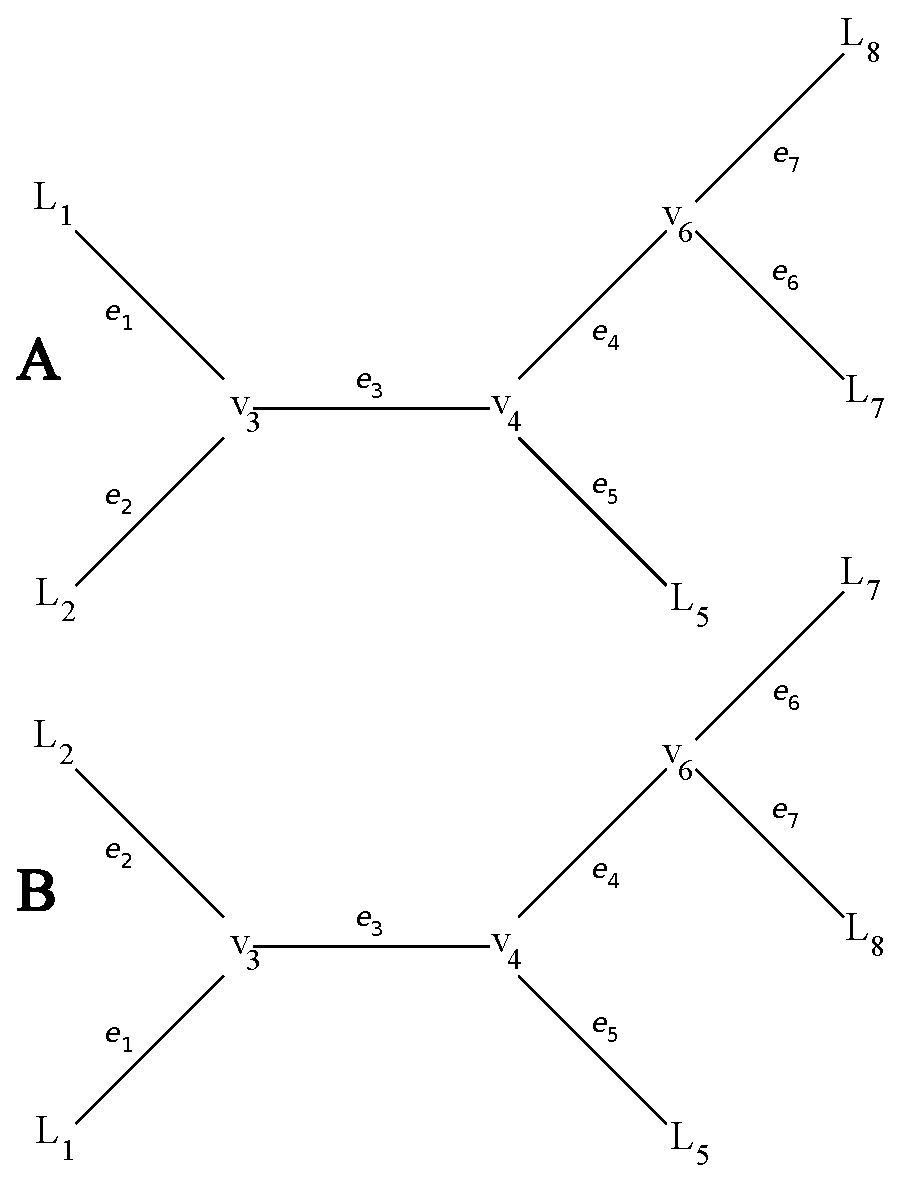
\includegraphics[scale=0.60]{figures/tut3/undirected_graph_topologies.eps}}
      {\caption[\textit{Grafos}]{Dois grafos (\textbf{A} e \textbf{B}) com a mesma topologia expressa pelas relações entre vértices (\textit{i.e.}, \textbf{V}), terminais (\textit{i.e.}, \textbf{L}) e arestas (\textit{i.e.}, \textbf{\texttt{e}}).}\label{tut3:fig:graph}}
  \end{figure}

%%%%%%%%%%%%%%%%%%%%%%%%%%% FIM DA FIGURA FLAT %%%%%%%%%%%%%%%%%%%%%

	Grafos são objetos matemáticos que consistem de um par de conjuntos (\textit{V/L},\textit{E}) de vértices (nós,\textit{V/L}) e arestas (ramos, \textit{E}; veja Figura \ref{tut3:fig:graph}). O \text{grau} de um vértice é o número de arestas conectados a ele. Desta forma, uma topologia binária $\textit{T} = (\textit{V/L},\textit{E})$ é um grafo conectado sem ciclos em que os terminais (\textit{L}) são vértices de grau 1 ao passo que os nós são vértices de grau 3. 

%%%%%%%%%%%%%%%%%%%%%%%%%%% FIGURA FLAT %%%%%%%%%%%%%%%%%%%%%%%%%%%
%  \vspace{-1em}
  \begin{figure}[H]
  \centering
    %\ffigbox[\FBwidth]
       \centering
      {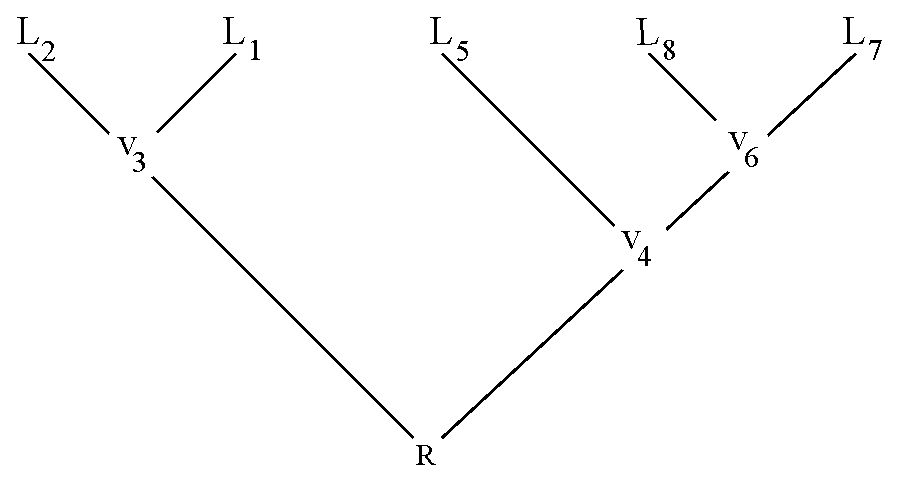
\includegraphics[scale=0.60]{figures/tut3/directed_graph.eps}}
      {\caption[\textit{Grafos}]{Grafo acíclico direcionado. Direcionamento é dado pela raiz (\textbf{R}), único vértice de graus 2.}\label{tut3:fig:rooted_graph}}
  \end{figure}

%%%%%%%%%%%%%%%%%%%%%%%%%%% FIM DA FIGURA FLAT %%%%%%%%%%%%%%%%%%%%%
	
O enraizamento de uma topologia binária (Figura \ref{tut3:fig:rooted_graph}) se da pela inserção de um vértice de grau 2 (\textit{i.e.}, \textbf{\texttt{R}}). Consequentemente, diagramas enraizados possuem um vértice e uma aresta adicional. Diagramas binários não-enraizados possuem ainda algumas propriedades matemáticas que devem ser conhecidas. A primeira delas é que o número de vértices internos é igual a $|L|-2$. A segunda é que o número de arestas (\textit{i.e.}, ramos) é igual a $2*|L|-3$. Finalmente, o número de topologias possíveis é uma função de $|L|$, ou seja, número de terminais. Portanto, o conjunto de topologias pode ser enumerado.
	
\subsection{Enumeração}\label{tut3:context:enumeration}
Em matemática e na ciência da computação, enumeração é a lista de todos os elementos de um conjunto. Em cladística, o termo é aplicado em buscas exatas no qual todas as topologias possíveis são avaliadas (ver Tutorial \ref{tut4}). A enumeração de topologias binárias não-enraizadas obedecem a seguinte fórmula:

\begin{center}
	para $n\geq3\colon\frac{(2n-4)!}{(n-2)!2^{n-2}}$
\end{center}
	
	O número de topologias enraizadas pode ser calculado multiplicando essa a fórmula acima pelo o número de ramos $(2n-3)$ ou incrementado $n$ por 1 (veja Tabela \ref{tut3:table:enumeration}).



%%%%%%%%%%%%%%%%%%%%%%%%%%% TABELA DE PARA ENUMERATION %%%%%%%%%%%%%%%%%%%%%%%%%%% 
%\begin{landscape}
\pagestyle{fancy}
\begin{center}

\begin{longtable}{lcccccc}
\caption[Tabela \ref{tut3:table:enumeration}: Enumeração de topologias]{Número de topologias binárias em função do número de terminais (\textit{i.e.}, $n$).} \label{tut3:table:enumeration} \\


\hline\hline  \textbf{$n$} & \textbf{não-enraizada} & \textbf{enraizada}\\
\hline
\endfirsthead

\multicolumn{3}{c}{{\bfseries \tablename\ \thetable{} -- Continuação.}}\\
\hline\hline \textbf{$n$} & \textbf{não-enraizada} & \textbf{enraizada}\\

\endhead
%\hline \multicolumn{3}{r}{{--continua na próxima página}} \\ \hline
%\endfoot
\hline \hline
%\hline \multicolumn{6}{l}{Consulte a página \url{http://wiki.linuxquestions.org/wiki/Linux_software_equivalent_to_Windows_software}.}
\endlastfoot
3 & 1 & 3\\
4 & 3 & 15\\
5 & 15 & 105\\
6 & 105 & 945\\
7 & 945 & 10395\\
8 & 10395 & 135135\\
9 & 135135 & 2027025\\
10 & 2027025 & 34459425\\
11 & 34459425 & 654729075\\
12 & 654729075 & 13749310575\\
13 & 13749310575 & 316234143225\\
14 & 316234143225 & 7905853580625\\
15 & 7905853580625 & 213458046676875\\

\end{longtable}
\end{center}
%\end{landscape}

%%%%%%%%%%%%%%%%%%%%%%%%%%% FIM DA TABELA ENUMERATION %%%%%%%%%%%%%%%%%%%%%%%%%%

Como pode ser observado, o número de topologias incrementa exponencialmente à medida que adicionamos terminais. Neste tutorial, o número de diagramas binários é um dos parâmetros que define o espaço de topologias (\textit{i.e.}, \textit{tree space}). Observe que até este momento, estas topologias são simplesmente objetos matemáticos, cujas características são relevantes para análises filogenéticas. A transição entre estes objetos e o conceito de teste de hipóteses requer análise de mérito relativo destes objetos. O mérito relativo depende de como esses modelos explicam nossas observações. Desta, a transição entre objetos meramente matemáticos (``\textit{tree-shaped-objects}'', senso \cite{Wheeler_2012}) e sua qualidade relativa para explicar (\textit{i.e.}, distribuição de caracteres) irá depender da implementação de critérios de otimalidade -- o que será explicado no próximo tutorial.


\section{Explorando o espaço de topologias}\label{tut3:tree_space_expĺore}

A seguir, vamos explorar alguns conceitos relacionados com o espaço de topologias. Iremos fazer uma série de execuções do \textit{script} \texttt{tree\_space.py} e é importante que ao executá-las, você tome nota dos resultados (uma opções é salvas as figuras geradas), pois você deverá compará-los à medida em que vai respondendo os exercícios. Este \textit{script} possui três rotinas básicas que serão explicadas no decorrer deste tutorial (Figura \ref{tut3:fig:prompt}).

%%%%%%%%%%%%%%%%%%%%%%%% FIGURA PROMPT %%%%%%%%%%%%%%%%%%%%%%%%
%  \vspace{-1em}
  \begin{figure}[H]
  \centering
    %\ffigbox[\FBwidth]
       \centering
      {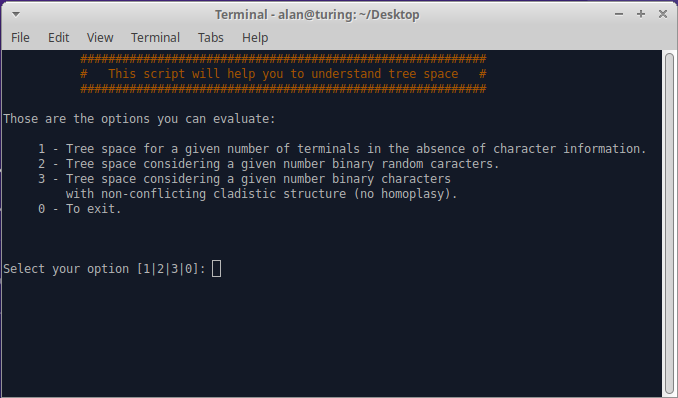
\includegraphics[scale=0.60]{figures/tut3/tree_space_prompt.png}}
      {\caption[Opções de \texttt{tree\_space.py}]{Opções de \texttt{tree\_space.py}. Veja texto abaixo para a descrição de cada uma dessas opções.}\label{tut3:fig:prompt}}
  \end{figure}
%%%%%%%%%%%%%%%%%%%%%%%% FIM DA FIGURA PROMPT %%%%%%%%%%%%%%%%%%


\subsection{Opção 1}\label{tut3:subs:flat}
Iremos iniciar avaliando como o número de terminais afeta o espaço de topologias na ausência de informação provinda de caracteres cladísticos. Na opção 1, este \textit{script} avalia todas as topologias possíveis (\textit{i.e.}, grafos binários) para determinado número de terminais $\ge 4 \le 10$\footnote{não exceda o limite superior desta rotina, pois o resultado demorará muito.}. Se você selecionar a opção 1 e pedir para o \textit{script} avaliar o espaço de topologias para 5 terminais você deverá obter dois gráficos representados da Figura \ref{tut3:fig:flat}.
 

%%%%%%%%%%%%%%%%%%%%%%%%%%% FIGURA Opt 1 %%%%%%%%%%%%%%%%%%%%%%%%%%%
%  \vspace{-1em}
  \begin{figure}[H]
  \centering
    %\ffigbox[\FBwidth]
       \centering
      {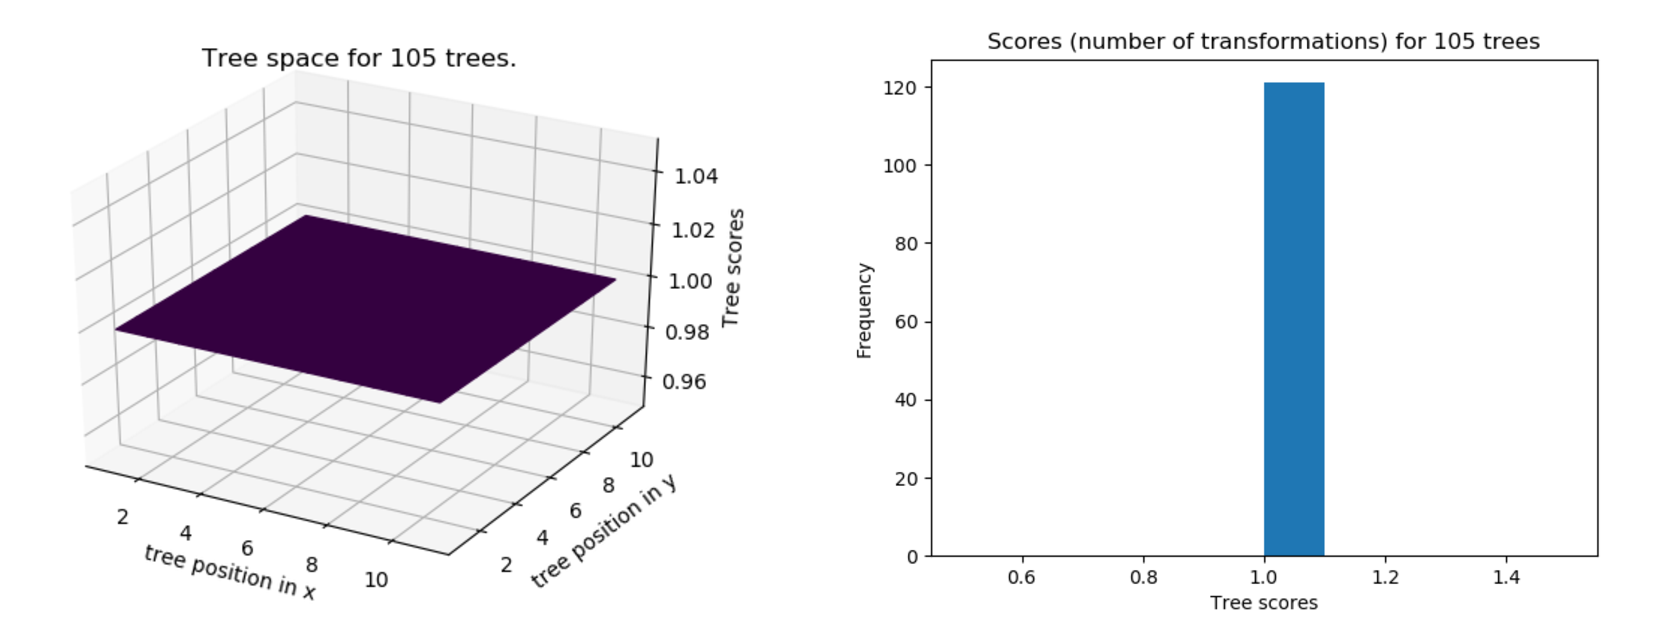
\includegraphics[scale=0.65]{figures/tut3/opcao_1_6_terminals.pdf}}
      {\caption[\textit{\textit{No informative characters} }]{Gráficos associados à opção 1 considerando 6 terminais sem informação cladística. À direita você encontra o custo de todas as topologias e à direita a frequência de distribuição destes custos.}\label{tut3:fig:flat}}
  \end{figure}

%%%%%%%%%%%%%%%%%%%%%%%%%%% FIM DA FIGURA Opt 1 %%%%%%%%%%%%%%%%%%%%%


Nesta figura, à direita você encontra um gráfico no qual o eixos $x$ e $y$ representam as coordenadas de todas as topologias geradas e no eixo $z$ seus respectivos custos  (\textit{Scores})\footnote{O ``custo'' refere-se ao número de transformações de estado de caráter para cada topologia.}. Ao lado direito desta figura, há um histograma mostrando a distribuição dos custos das topologias encontradas.\\

\stepcounter{ex}
\begin{blackBlock}{\textbf{Exercicio 3.\arabic{ex}}}\label{tut3:ex:3.\arabic{ex}}
	Considere estes gráficos como uma representação aproximada da complexidade do espaço de topologias. Faça algumas execuções deste \textit{script} variando o número de terminais e responda:
\begin {myindentpar}{0.5cm}
\begin{enumerate}[\itshape i.]
 \item{Há um único parâmetro deste espaço que é afetado pelo número de terminais. Qual seria esse parâmetro e de que forma o espaço de topologias está variando?}\label{tut3:ex1}\\
  \begin{center}
  \line(1,0){400}\\
  \line(1,0){400}\\
  \line(1,0){400}\\
  \end{center}

\end{enumerate}
\end{myindentpar}

\end{blackBlock}

Como você pode observar, os custos de todas as topologias são idênticos. No entanto, considere a Figura \ref{tut3:fig:enumeration_indexed}.

%%%%%%%%%%%%%%%%%%%%%%%%%%% FIGURA ENUM %%%%%%%%%%%%%%%%%%%%%%%%%%%
%  \vspace{-1em}
  \begin{figure}[H]
    %\ffigbox[\FBwidth]
       \centering
      {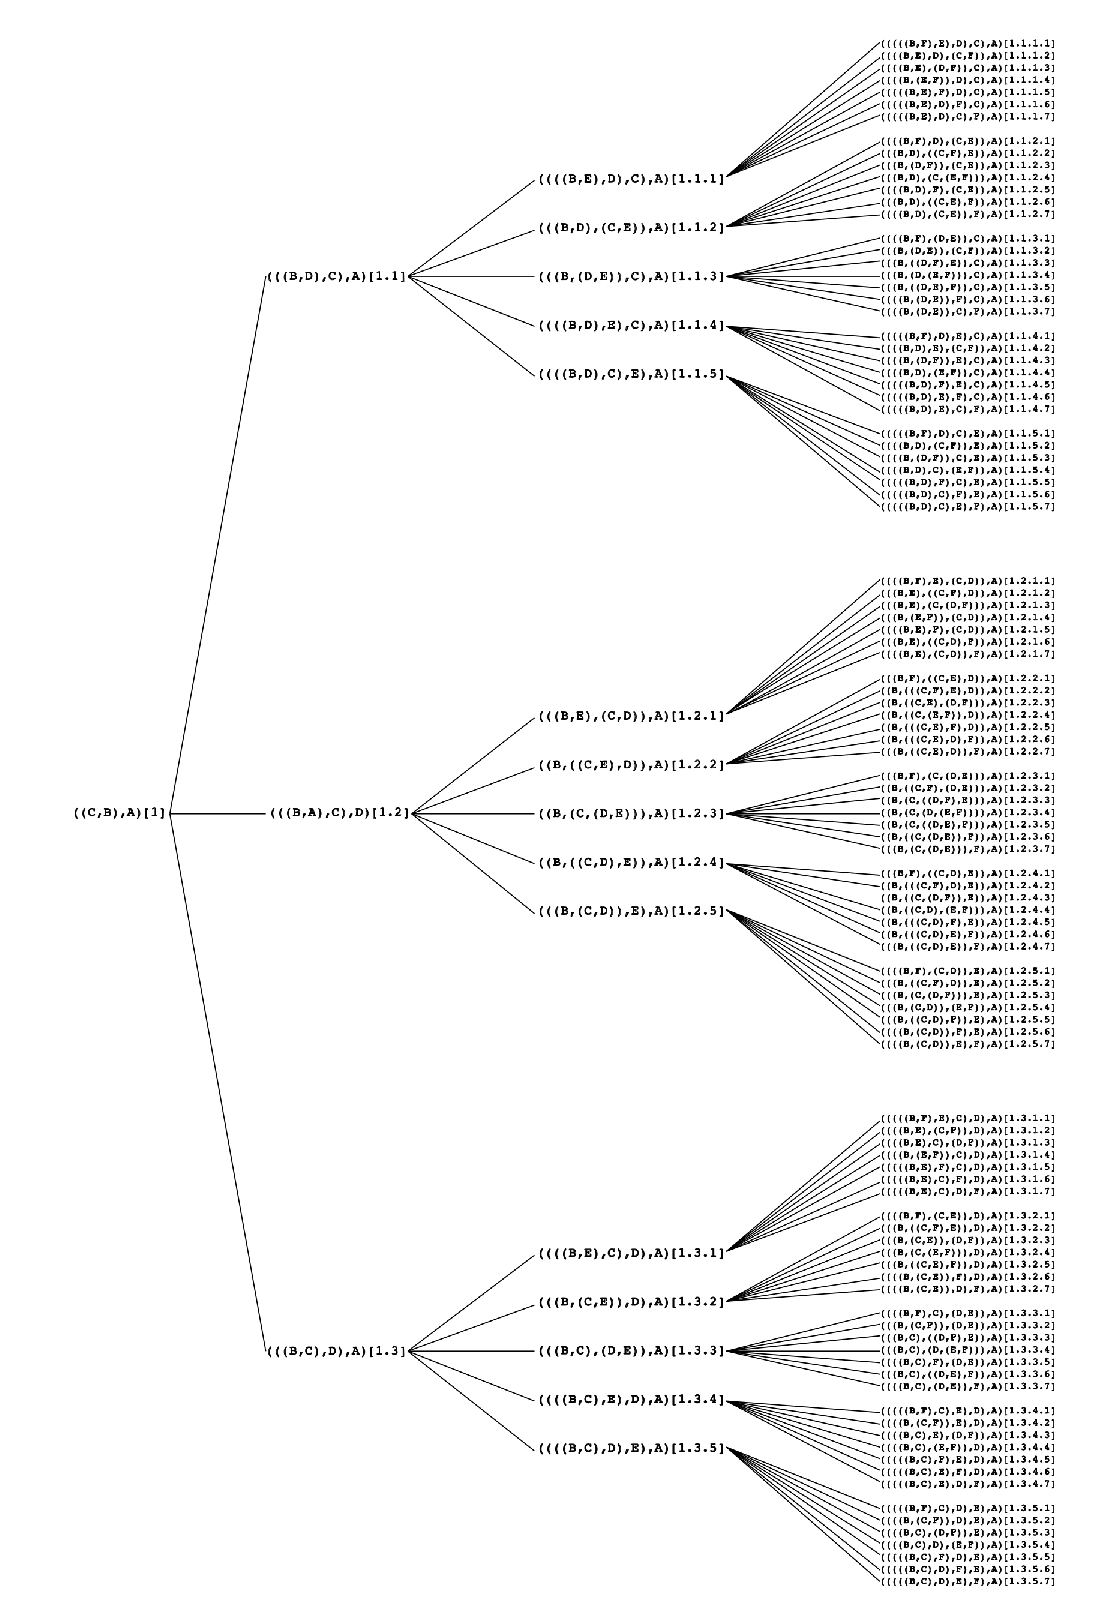
\includegraphics[scale=0.80]{figures/tut3/enumeration_A4.eps}}
      {\caption[Enumeração indexada]{Enumeração das topologias para 6 terminais indexadas segundo o arquivo \texttt{06\_enumeration.tre}. Observe a lógica de indexação desta topologia pelos dígitos entre colchetes (\textit{i.e.}, \texttt{[1.3.5.1]}).}\label{tut3:fig:enumeration_indexed}}
  \end{figure}

%%%%%%%%%%%%%%%%%%%%%%%%%%% FIM DA FIGURA ENUM %%%%%%%%%%%%%%%%%%%%%

Observe que essas tolologias divergem à medida em que se afastam da topologia inicial (\textit{i.e.}, \texttt{[1]}). É evidente que nosso primeiro exercício não detecta este componente do espaço de árvores. No entanto, isso seria possível avaliando a distância topológica de acordo com alguma outra métrica.\\

\textcite{Robinson_and_Foulds_1981} foram uns dos primeiros a propor uma métrica que avaliasse diferença entre árvores filogenéticas. Os detalhes do cálculo de distância são irrelevantes para os propósitos deste turorial, mas o leitor mais curioso deve consultar o artigo de \textcite{Robinson_and_Foulds_1981} e \textcite{BogdanowiczETGiaro_2013} para maiores detalhes (no diretório \texttt{literature} anexo a este tutorial). Via de regra, métricas que computam distâncias entre topologicas consideram os passos necessários, de acordo com algum critério, para tranformar uma topologia em outra. Neste tutorial iremos avaliar distâncias entre topologias utilizando o \href{http://www.ib.usp.br/grant/anfibios/researchSoftware.html/}{YBYRÁ}, que usa a métrica proposta por \textcite{Robinson_and_Foulds_1981}.\\

O uso do UBYRÁ para este propósito é relativamente simple. Suponha, por exemplo, que eu queira avaliar a distância entre a topologia \texttt{[1.1.1.1]} e as demais topologias enumeradas a partir de \texttt{[1.1.1]}. Os passos a seguir seriam:

\begin {myindentpar}{0.5cm}
\begin{enumerate}[\itshape i.]
	\item{} Extrair as topologias desta família (\textit{i.e.}, \texttt{[1.1.1]} do arquivo \texttt{06\_enumeration.tre}. A forma mais simples de fazer isso seria utilizar a seguinte linha de comando:

\shellcmd{egrep '\textbackslash[1\textbackslash.1\textbackslash.1\textbackslash..*' 06\_enumeration.tre > 1.1.1.n.tre}

	\item{} Extrair a topologia \texttt{1.1.1.1.tre} de \texttt{1.1.1.n.tre} com a seguinte linha de comando:

\shellcmd{head -n 1 1.1.1.n.tre > 1.1.1.1.tre}

	\item{} Criar o arquivo de configuração necessário para executar o \href{http://www.ib.usp.br/grant/anfibios/researchSoftware.html/}{YBYRÁ}. Para computar as distâncias entre a topologia \texttt{1.1.1.1.tre} e as demais topologias em \texttt{1.1.1.n.tre}, o arquivo de configuração (\textit{e.g.}, \texttt{conf.txt}) deve ter o seguinte conteúdo:

\begin{lstlisting}[label=tut3:config1]
>id = CalcDist_6a
<begin files
        1.1.1.1.tre;
        1.1.1.n.tre;
end files>
>n = 1 [1.1.1.1.tre]
>opt = 3
>compare = 1
>root=A
>verbose
\end{lstlisting}

Neste arquivo de configuração, a linha 1 define a ID (identidade) da análise. As linhas 2 a 5 definem os arquivos que contém as topologias a serem comparadas. A linha 6 define a topologia de referência. As linhas 7 e 8 configuram o tipo de comparação que o programa irá executar (veja documentação do programa para maiores detalhes). A linha 9 informa o táxon de enraizamento -- necessário para computar as distâncias. Finalmente, a linha 10 configura o programa para informar ao usuário as etapas que estão sendo executadas à medida em que o programa prossegue.

	\item{} Executar o \href{http://www.ib.usp.br/grant/anfibios/researchSoftware.html/}{YBYRÁ} da seguinte forma:

\shellcmd{python ybyra\_sa.py -f conf.txt}\\

	Após a execução do programa, você deverá obter, dentre várias linhas de saida, a seguinte informação:

\texttt{The file MATRIX\_calcDist\_6a.txt was created}.\\

Este arquivo contém os resultados que deseja e estão sumarizados na Tabela \ref{tut3:table:dist}.

%%%%%%%%%%%%%%%%%%%%%%%%%%% TABELA DE PARA ENUMERATION %%%%%%%%%%%%%%%%%%%%%%%%%%% 
%\begin{landscape}
\pagestyle{fancy}
\begin{center}

\begin{longtable}{ccccccc}
\caption[Tabela \ref{tut3:table:dist}: Cálculo de distância topológica]{Distâncias topológicas de acordo com \textcite{Robinson_and_Foulds_1981}. \textbf{SC}, Clados compartilhados (\textit{i.e.}, comuns entre as duas topologias). \textbf{CC}, Clados combinados (\textit{i.e.}, soma de todos os clados distintos encontrados em ambas topologias). \textbf{LD}, Distância local. } \label{tut3:table:dist} \\


\hline\hline \textbf{Tree No.} & \textbf{Tree No.} & \textbf{SC} & \textbf{CC} & \textbf{LD = $1-(\frac{SB}{CB})$}\\
\hline
\endfirsthead

\multicolumn{3}{c}{{\bfseries \tablename\ \thetable{} -- Continuação.}}\\
\hline\hline \textbf{Tree No.} & \textbf{Tree No.} & \textbf{SC} & \textbf{CC} & \textbf{LD = $1-(\frac{SB}{CB})$}\\

\endhead
%\hline \multicolumn{3}{r}{{--continua na próxima página}} \\ \hline
%\endfoot
\hline \hline
%\hline \multicolumn{6}{l}{Consulte a página \url{http://wiki.linuxquestions.org/wiki/Linux_software_equivalent_to_Windows_software}.}
\endlastfoot
1 & 2 & 5 & 5 & 0\\
1 & 3 & 2 & 8 & 0.75\\
1 & 4 & 3 & 7 & 0.57\\
1 & 5 & 4 & 6 & 0.33\\
1 & 6 & 4 & 6 & 0.33\\
1 & 7 & 3 & 7 & 0.57\\
1 & 8 & 2 & 8 & 0.75\\

\end{longtable}
\end{center}
%\end{landscape}

%%%%%%%%%%%%%%%%%%%%%%%%%%% FIM DA TABELA ENUMERATION %%%%%%%%%%%%%%%%%%%%%%%%%%

\end{enumerate}
\end{myindentpar}

\stepcounter{ex}
\begin{blackBlock}{\textbf{Exercicio 3.\arabic{ex}}}\label{tut3:ex:3.\arabic{ex}}
	Com base no exemplo acima, no qual foram calculadas as distâncias entre topologias responda:
\begin {myindentpar}{0.5cm}
\begin{enumerate}[\itshape i.]
 \item{Como se comportam as distâncias entre a topologia \texttt{1.1.1.1.tre} e aquelas enumeradas para as demais famílias (\textit{i.e.}, \texttt{1.1.2} e \texttt{1.1.3})?}\label{tut3:ex2}\\
  \begin{center}
  \line(1,0){400}\\
  \line(1,0){400}\\
  \end{center}

 \item{O tamanho do espaço de topologias influencia os resultados que você obteve no item anterior? (\textbf{OBS.}: considere que há topologias enumeradas para 7, 8, 9 2 10 terminais.)}\label{tut3:ex2}\\
  \begin{center}
  \line(1,0){400}\\
  \line(1,0){400}\\
  \end{center}

\end{enumerate}
\end{myindentpar}

\end{blackBlock}


%%%%%%%%%%%%%%%%%%%%%%%%%%% FIGURA Opt 2 %%%%%%%%%%%%%%%%%%%%%%%%%%%
%  \vspace{-1em}
  \begin{figure}[H]
  \centering
    %\ffigbox[\FBwidth]
       \centering
      {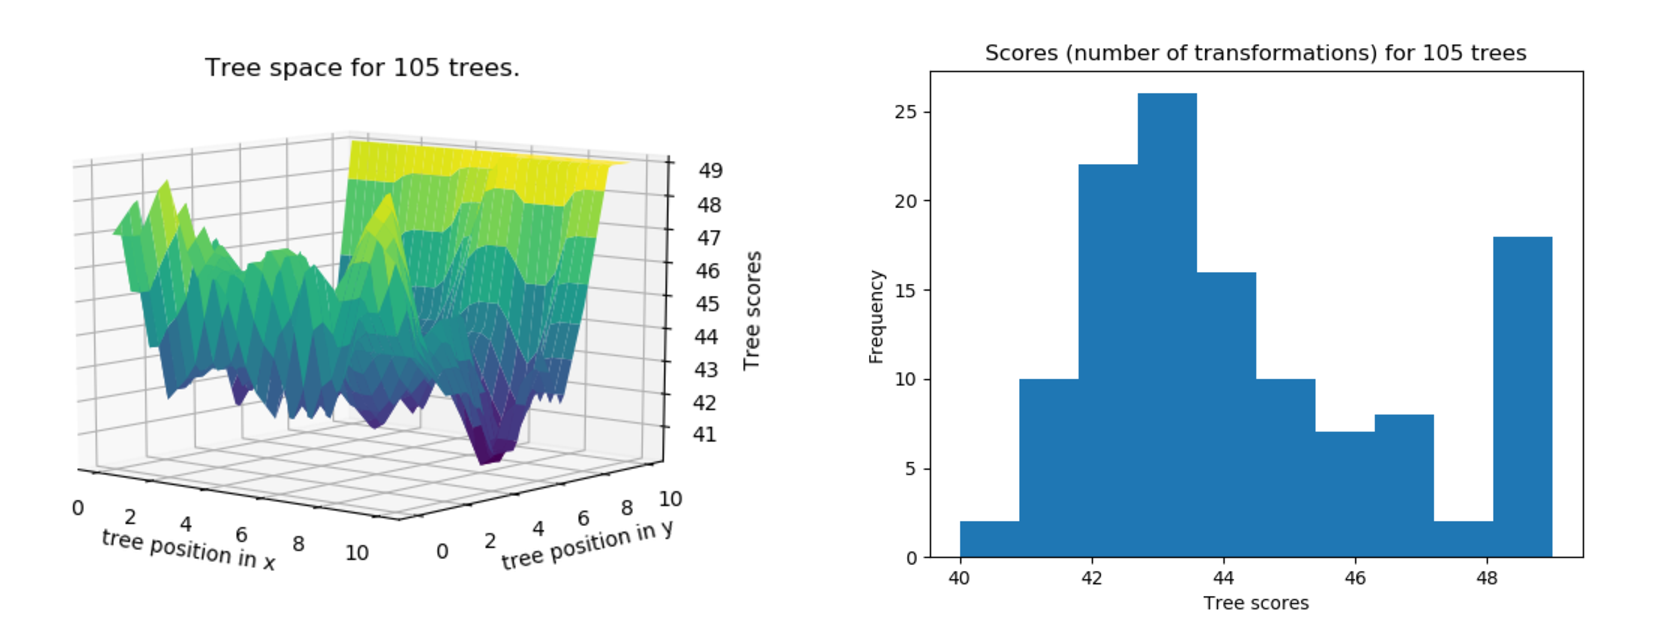
\includegraphics[scale=0.65]{figures/tut3/opcao_2_6_terminals_24_characters.pdf}}
      {\caption[\textit{\textit{Random space} }]{Gráficos associados à opção 2 considerando 6 terminais e 24 caracteres aleatórios. À direita você encontra o custo de todas as topologias e à direita a frequência de distribuição destes custos.}\label{tut3:fig:rand}}
  \end{figure}

%%%%%%%%%%%%%%%%%%%%%%%%%%% FIM DA FIGURA OIpt 2 %%%%%%%%%%%%%%%%%%%%%


\subsection{Opção 2}\label{tut3:subs:rand}
A opção 2 faz com que o \textit{script} proceda da seguinte forma (Figura \ref{tut3:fig:rand}). Dado o número de terminais e caracteres, \texttt{tree\_space.py} gera uma matriz aleatória com $n$ caracteres binários cuja probabilidade de $0$ ou $1$ é igual a $0.50$. Esta matriz de dados é submetida ao programa TNT para computar o custo de todas a topologias possíveis dado o número de terminais.\\


%%%%%%%%%%%%%%%%%%%%%%%%%%% FIGURA RAND %%%%%%%%%%%%%%%%%%%%%%%%%%%
%  \vspace{-1em}
  \begin{figure}[H]
  \centering
    %\ffigbox[\FBwidth]
       \centering
      {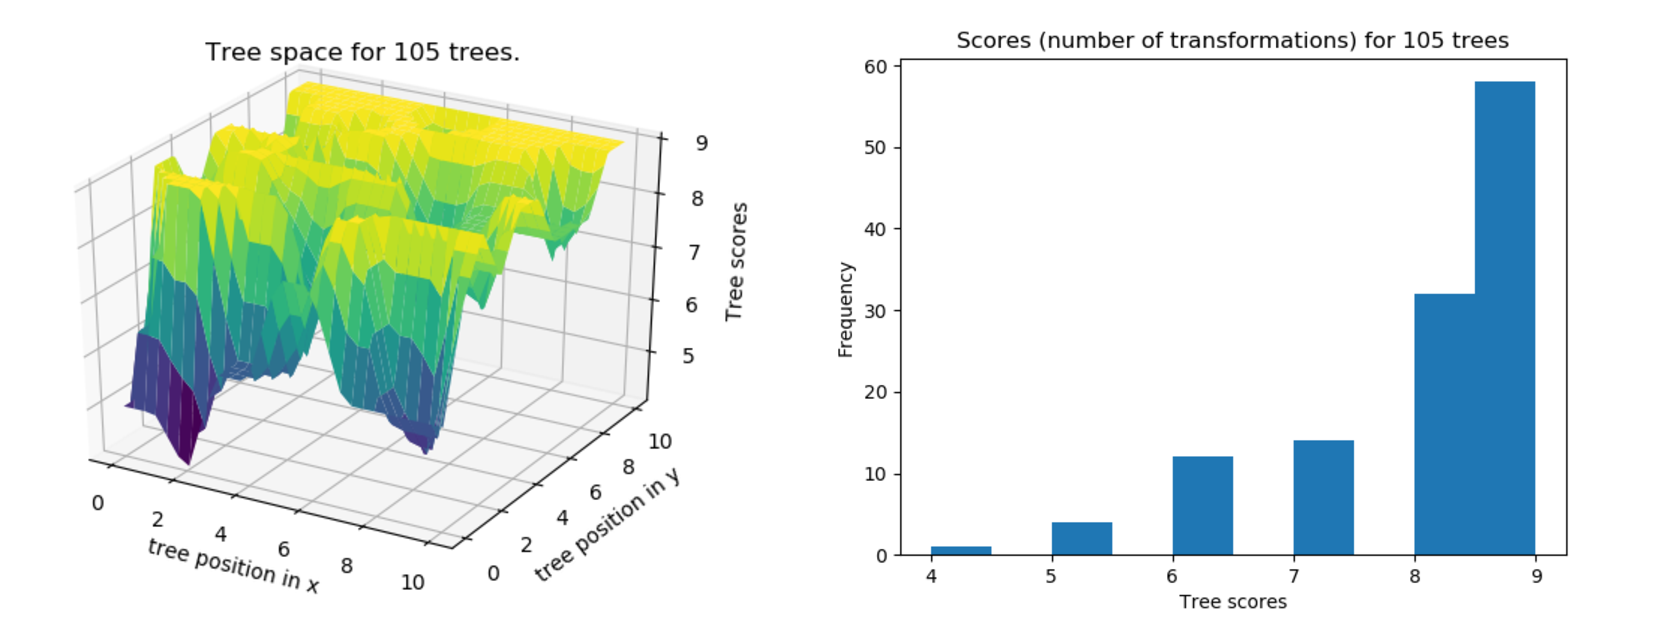
\includegraphics[scale=0.65]{figures/tut3/opcao_3_6_terminals_24_characters.pdf}}
      {\caption[\textit{\textit{Structured space} }]{Gráficos associados à opção 2 considerando 6 terminais e uma matriz de representação (sem homoplasias). À direita você encontra o custo de todas as topologias e à direita a frequência de distribuição destes custos.}\label{tut3:fig:struc}}
  \end{figure}

%%%%%%%%%%%%%%%%%%%%%%%%%%% FIM DA FIGURA RAND %%%%%%%%%%%%%%%%%%%%%


\subsection{Opção 3}\label{tut3:subs:struc}
Esta rotina difere da anterior em alguns pontos importantes (Figura \ref{tut3:fig:struc}). Ao definir o número de terminais, \texttt{tree\_space.py} gera uma topologia aleatória e uma matriz de representação. Por esta razão, não há como definir o número de caracteres, pois estes são dependentes dos números de nós da topologia binária para os quais a matriz de representação dará suporte. Posteriormente, TNT avalia o custo desta matriz de representação em relação ao universo de enumeração de todas as topologias binárias. \\

\stepcounter{ex}
\begin{blackBlock}{\textbf{Exercício 3.\arabic{ex}}}\label{tut3:ex:3.\arabic{ex}}
	Você deverá fazer uma série de execuções das opções 2 e 3. Compare os resultados salvando as figuras se considerar necessário. Com base nos seus resultados, responda:
\begin {myindentpar}{0.5cm}
\begin{enumerate}[\itshape i.]
 \item{Como se comporta o espaço de topologias em ambas as rotinas?}\label{tut3:ex3}\\
  \begin{center}
  \line(1,0){400}\\
  \line(1,0){400}\\
  \line(1,0){400}\\
  \end{center}

 \item{O comportamento dos valores de custo mínimo direfem entre as duas rotinas?}\\
  \begin{center}
  \line(1,0){400}\\
  \line(1,0){400}\\
  \end{center}

 \item{Qual é a observação mais relevante que você observa com relação aos histogramas produzidos por essas duas rotinas?}\\
  \begin{center}
  \line(1,0){400}\\
  \line(1,0){400}\\
  \line(1,0){400}\\
  \end{center}

 \item{Como você obteve algum resultado da opção 2 que resultou em uma única topologia com o menor custo? Você acha isso relevânte para inferência filogenética?}\\
  \begin{center}
  \line(1,0){400}\\
  \line(1,0){400}\\
  \end{center}

\end{enumerate}
\end{myindentpar}

\end{blackBlock}



\vspace{20pt}

\stepcounter{ex}
\begin{blackBlock}{\textbf{Exercicio 3.\arabic{ex}}}\label{tut3:ex:3.\arabic{ex}}
	Abaixo, defina o que você entende por espaço de topologia e quais são o elementos que afetam sua conformação:
  \begin{center}
  \line(1,0){400}\\
  \line(1,0){400}\\
  \line(1,0){400}\\
  \line(1,0){400}\\
  \line(1,0){400}\\
  \line(1,0){400}\\
  \line(1,0){400}\\
  \line(1,0){400}\\
  \line(1,0){400}\\
  \line(1,0){400}\\
  \line(1,0){400}\\
  \line(1,0){400}\\
  \line(1,0){400}\\
  \line(1,0){400}\\
  \line(1,0){400}\\
  \line(1,0){400}\\
  \line(1,0){400}\\
  \line(1,0){400}\\
  \line(1,0){400}\\
  \line(1,0){400}\\
  \line(1,0){400}\\
  \line(1,0){400}\\
  \line(1,0){400}\\
 
 \end{center}


\end{blackBlock}


%%%%%%%%%%%%%%%%%%%%%%%%%%%% HERE ENDS TEXT AND ADDS REFERENCES %%%%%%%%%%%%%%%%%%%%%%%%%%%% 
\section{Referências}\label{tut3:refs}
\printbibliography[heading=none]
\end{refsection}
%